\documentclass{beamer}
\usepackage{pgfpages}
\usepackage{url}
\usepackage[round]{natbib}
\usepackage{makecell}
\usepackage{booktabs}
\usepackage{pifont}

\setbeameroption{show notes on second screen}
\setbeamertemplate{caption}[numbered]

\urldef{\repository}\url{https://github.com/julianbarg/oil_industry/}
\urldef{\pipelinesDashboard}\url{https://julianbarg.shinyapps.io/pipelines_dashboard/}
\urldef{\incidentDashboard}\url{https://julianbarg.shinyapps.io/incident_dashboard/}
\urldef{\incidentDefinition}\url{https://www.phmsa.dot.gov/data-and-statistics/pipeline/pipeline-incident-20-year-trends}

\title{Valuing Peace and Quiet: the Effect of Expansion Mode on Learning toward Subordinate Goals}
\author{Julian Barg}
\institute{Ivey Business School}
\date{Sept 27, 2019}
\logo{
\includegraphics[scale=0.08]{resources/ivey_logo.jpg}}
\begin{document}
	
\frame{\titlepage}

\begin{frame}
	\frametitle{Outline}
	\tableofcontents
\end{frame}

\begin{frame}
	\repository
	\note{Includes data collection, variable transformation, stata code for results, and even this presentation, and the dashboards.}
\end{frame}

\begin{frame}
	\frametitle{Summary}
	\begin{block}{Findings}
		\begin{itemize}
			\item Organization-wide strategic changes will disrupt learning that has occurred in suborganizations.
			\note{This is what expansion mode refers to in the title, not greenfield or M\&A (although there are M\&As in the dataset).\\\medskip}
			\item Thus, when "nothing happens", something does happen: organizational learning.
			\item From a learning perspective, it is better to take a long-term perspective on strategic adjustments.
				\begin{itemize}
					\item Implementing change in a less disruptive fashion.
				\end{itemize}
				\note{"Learning perspective" matters, because from a technology perspective, the conclusion might be different.}
			\item Depending on the context, implications for organizational performance (environmental and economic).
			\note{In a temporality-inspired learning research fashion. Depending on the type of organization - where mistakes threaten survival, very relevant.}
		\end{itemize}
	\end{block}
\end{frame}

\section{Context}

\begin{frame}
	\frametitle{Context}
	\pipelinesDashboard
	\note{"This is a tool I use for my research." Just briefly show the nature of the data.
		\begin{itemize}
			\item We have comprehensive data on pipelines in the US.
			\item We know which organizations have how many miles. (show top 5)
			\item We know how old their pipelines are.
			\item We know how many incidents occur.
			\item So it would be a great context to study strategy, and how it affects incident rates.
		\end{itemize}}
\end{frame}

\begin{frame}
	\frametitle{Cases}
	\incidentDashboard
	\note{"This is a tool I use for my research." Just briefly show the scale, because i found it hard to imagine, just from numbers.
		\begin{itemize}
			\item Show all organizations at once, add some jitter, alpha.
			\item Show one group, remove jitter, alpha.
		\end{itemize}}
\end{frame}

\begin{frame}
	\frametitle{Context}
	\begin{block}{High-profile bankruptcies related to pipeline incidents}
		\begin{itemize}
			\item Greka Energy/HVI Cat Canyon (1996, 2005, 2019)
			\note{Greka: History of oil spills, settlements relatively unexpensive, e.g., \$12 million fine caused bankruptcy in 2019, ironically, CEO once stated company motto as "Working for profits".\medbreak}
			\item Pacific Gas and Electric Company (2001, 2019)
			\note{PG\&E: After 2010 explosion with 8 deaths, paid \$300m in fines, \$400m in refunds, \$850m for upgrades, and \$500m in settlements.\medbreak}
			\item{EdgeMark (2019)}
			\note{EdgeMark: Energy Transfer pipeline explosion led to EdgeMark Bankruptcy. Ontario Teachers' Pension fund held minority stake. \bigbreak}
		\end{itemize}	
	\end{block}

	\hrulefill
	
	$\rightarrow$ There is some relevance for traditional performance also.
	\note{\hrulefill \smallbreak
		I don't explore this relevance for performance any further though.}
\end{frame}


\begin{frame}
	\frametitle{Research Question}
	How does organizational learning and forgetting play out in the context of strategic adjustment and hierarchies?
	\note{Let me show you the phenomenon I have been working on, what I believe is going on, and how that generalizes.}
\end{frame}

\section{Learning}

\begin{frame}
	\frametitle{Organizational forgetting: Definitions}
	\begin{itemize}
		\item \textit{Organizational learning}: "change in the organization's knowledge that occurs as a function of experience" \citep[p. 31]{Argote2013}.
		\item \textit{Organizational forgetting}: "the loss, voluntary or otherwise, of organizational knowledge [which] often leads to a change in organizational capabilities because of the absence of some piece of knowledge" \citep[p. 1606]{DeHolan2004}.
		\note{Both forgetting and disruptions are thought to be sometimes positive, too, but I will not cover that here.\medbreak Disruption also sometimes desdribed as merely "interacting" with forgetting (Anderson \& Lewis 2014).\medbreak}
		\item \textit{Disruptions}: "organizational change-inducing events" \citep[p. 362]{Anderson2014}
		\note{Will have examples of disruptions in the next couple of slides.}
	\end{itemize}
\end{frame}

\begin{frame}
	\frametitle{\insertsection}
	\framesubtitle{Learning curve}
	\begin{figure}
		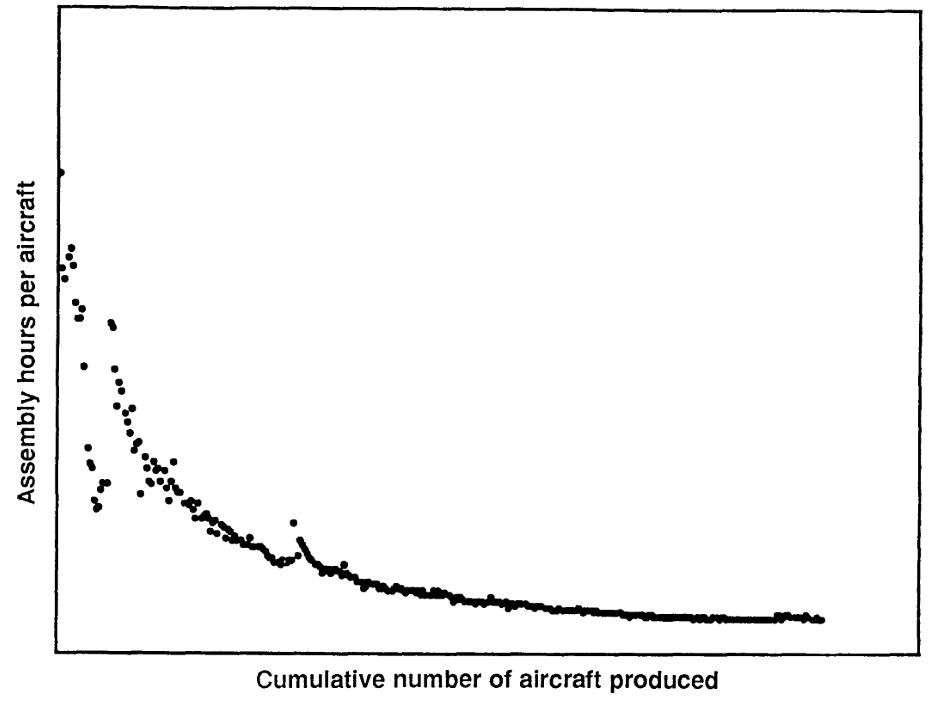
\includegraphics[height=5cm]{resources/learning_curve1.png}
		\caption{Relation between assembly hours per aircraft and cumulative number produced. Units omitted. From: \citet[p. 921]{Argote1990}}
		\note{You have probably seen this before. Read out caption. So in our context, we could imagine an organization operating its pipeline and equipment, getting better at it, making less mistakes, having less incidents. The organization in charge of pipeline safety is a suborganization.}
	\end{figure}
\end{frame}

\begin{frame}
	\frametitle{\insertsection}
	\framesubtitle{Disrupted learning}
	\begin{figure}
		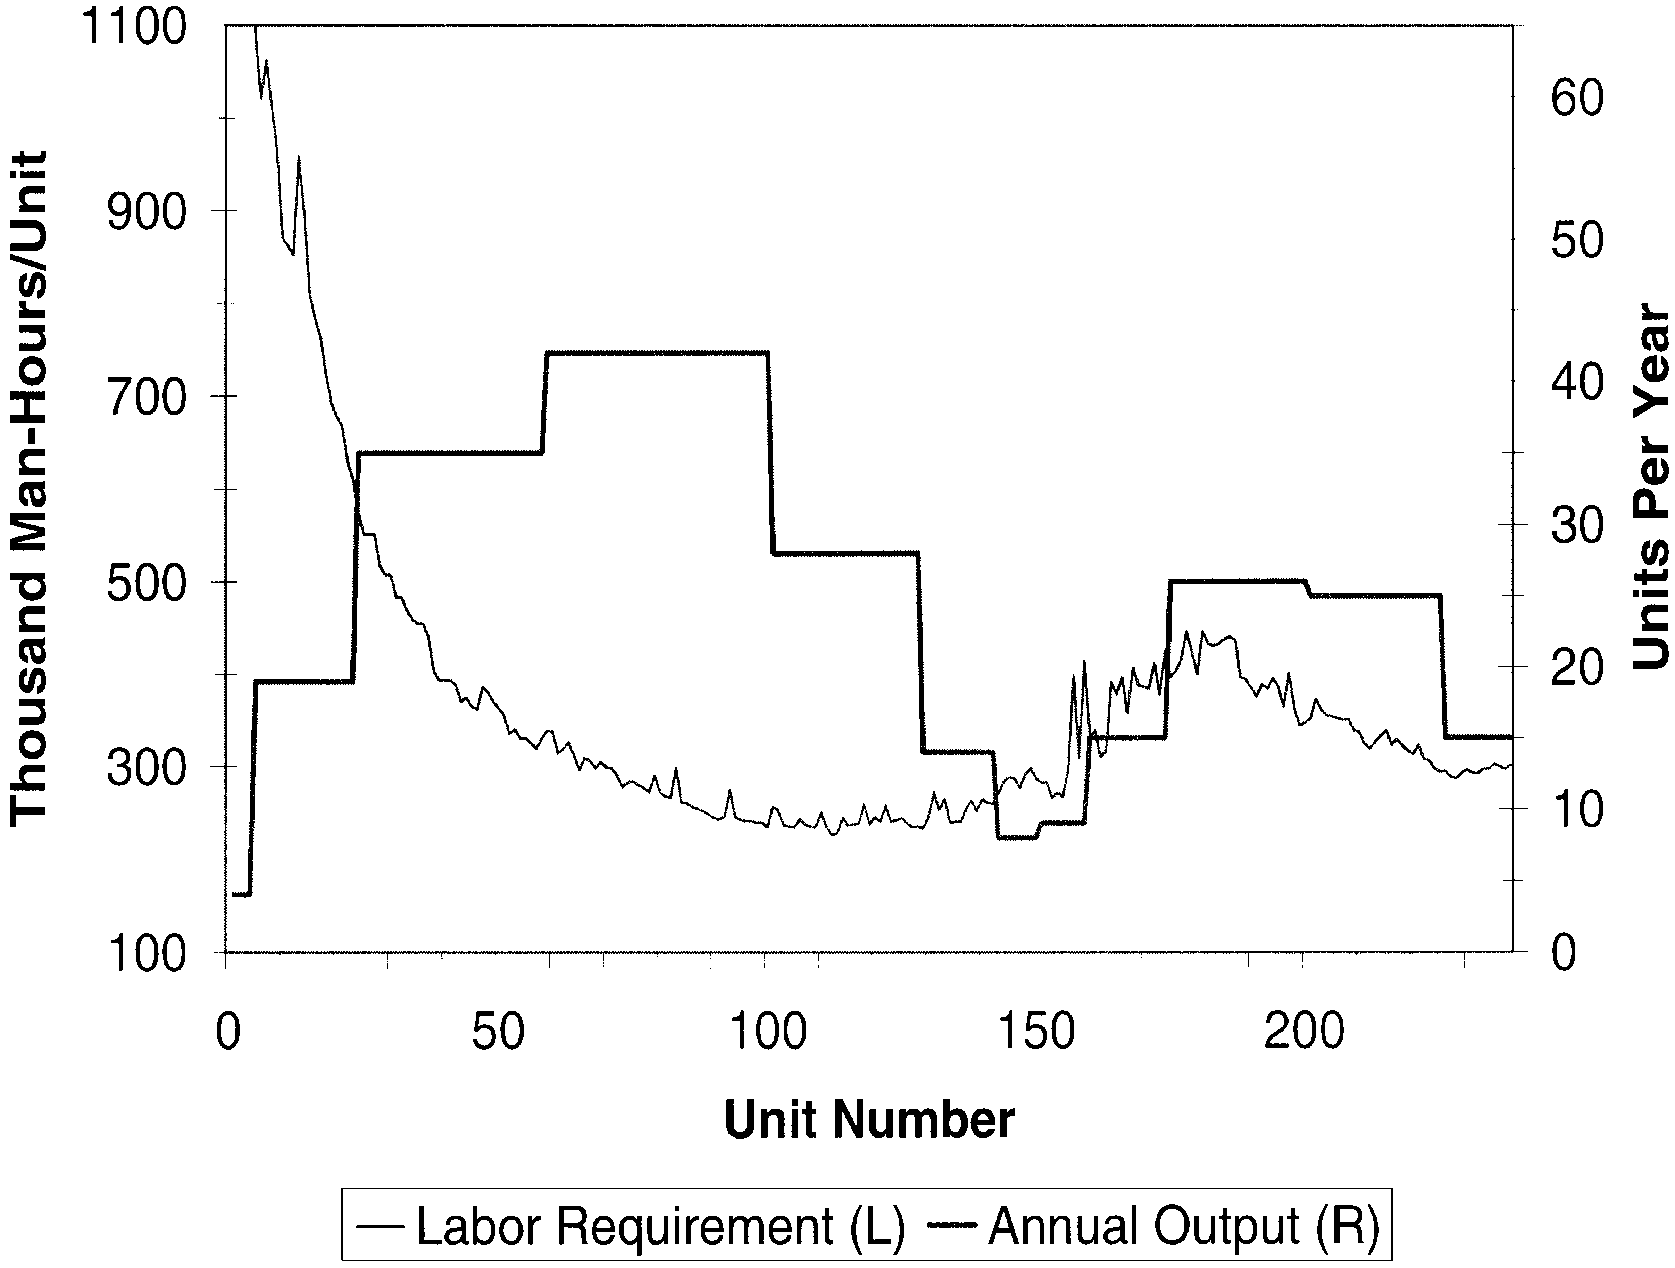
\includegraphics[height=5cm]{resources/learning_curve2.png}
		\caption{L-1011 Production: Direct Labor Requirement and Yearly Output. From: \citet[p. 1039]{Benkard2000}}
	\end{figure}
	\note{We see more than in the last picture. This is the production of the Lockheed L-1011. Famous for being an amazing plane, but a commercial failure. What happend here, around 150 units? Economic downturn, production was disrupted. Then, company decided the only way to break even is to produce a certain number of planes, but that did not happen.}
\end{frame}

\begin{frame}
	\frametitle{\insertsection}
	\framesubtitle{Disrupted learning}
	\begin{figure}
		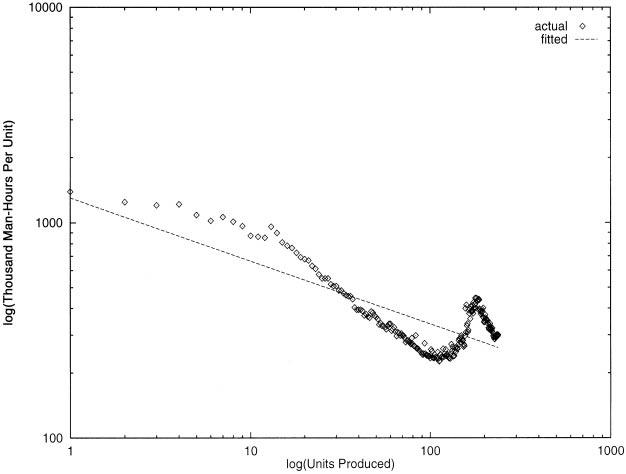
\includegraphics[height=5cm]{resources/learning_curve3.jpg}
		\caption{Traditional Learning Curve: All 238 (log-log). From: \citet[p. 1046]{Benkard2000}}
	\end{figure}
	\note{This is what actually happened. After Lockheed increased production again, the number of man-hours per plane actually increased for a while, before it decreased again. In our context, we could imagine a pipeline operator operating a pipeline for many years, then shutting it off for a while, before resuming operations. Knowledge would be lost, especially if the shut-off went hand in hand with lay-offs, and if the company had to hire new staff later.}
\end{frame}

\begin{frame}
	\begin{block}{}
		\Huge Organizational forgetting
		\bigbreak		
		\normalsize Also known as knowledge depreciation
		\note{The Lockheed is a pretty famous example for this.}
	\end{block}{}
\end{frame}

\begin{frame}
	\frametitle{Organizational forgetting}
	\begin{itemize}
		\item Turnover \citep{DeHolan2004,Rao2006}
		\note{Relate sources of forgetting to our context.\medbreak When a large number and/or key employees leave a company, and knowledge and/or networks are lost as a result. Which is also acknowledges in the wider learning literature.\medbreak}
		\item Loss of recorded knowledge
		\item Technology becoming irrelevant
		\item Decay of social networks \citep{Argote2013_3,Argote1990,Thompson2007}
		\item Disruption
		\item 
		\begin{itemize}
			\item Internal
				\begin{itemize}
					\item Disruption of regular production 
					\item Technology \citep{Amburgey1993,Edmondson2001}
					\item Restructuring/reorganization/layoffs (or even hirings) \citep{Benkard2000,Anderson2014}
				\end{itemize}
			\item External
				\begin{itemize}
					\item Economic cycles \citep{Rockart2019}
					\item Natural disasters \citep{Anderson2014}
				\end{itemize}
		\end{itemize}
	\end{itemize}
	\note{Organizational disruption is special case of organizational forgetting. Disruption can stem from inside, or outside of the organization.}
\end{frame}




\section{Hypothesis development}

\begin{frame}
	\Large So what do I think is happening in our context?
\end{frame}

\begin{frame}
	\frametitle{Hypothesis development}
	\begin{itemize}
		\item Organizations operate pipelines, part of the organization is in charge of safety.
		\note{Organization can be in the business of pipelines, or extraction. Usually a dedicated department in charge of pipeline safety.\medskip}
		\pause
		\item HQ makes strategic decisions that impact the whole organizations.
		\pause
		\item In many scenarios, the strategic decision can be a source of disruption.
		\note{For other parts of the organization.\medskip}
		\pause
		\item In the context of pipelines, we can track decision making very well, because we know the scope of the organization/suborganization company very well.
		\note{So that is what we are going to do. We track the scope of the organization, the expansion mode (sporadic or even across time), and the impact on pipeline safety.}
	\end{itemize}
\end{frame}

\begin{frame}
	\frametitle{Hypothesis development}
	\begin{block}{Hypothesis 1}
		Strategic adjustments from the parent organization disrupt the learning of suborganizations.
	\end{block}
	\pause
	
	\begin{block}{Hypothesis 2}
		Phases of stability, with less strategic adjustments being initiated by the parent organization, allow for the suborganizations to learn.
	\end{block}
	\pause
	
	\begin{block}{Hypothesis 1c \small (\textbf{C}ompeting)}
		Strategic adjustments act as external shocks to suborganizations, and induce additional learning.
	\end{block}
\end{frame}

\section{Methods}

\begin{frame}
	\frametitle{Before I forget...}
	\begin{itemize}
		\item Fixed-effect
		\item Company-year
	\end{itemize}
\end{frame}

\begin{frame}
	\frametitle{Independent variable}
	Change of the organization over time - pipeline assets.\smallbreak
	$\rightarrow$ \textbf{Low} if the organization is not changing, or changing at constant pace.\smallbreak
	$\rightarrow$ \textbf{High} if organization deviates from previous course.
	
	\hrulefill
	
	$A_{t} = ((C_{t} - \bar{C})^2 + (C_{t-1} - \bar{C})^2 + (C_{t-2} - \bar{C})^2) / 2$\smallbreak
	where\smallbreak
	$C = M_{t} - M_{t-1}$\smallbreak
	$M$ is \textbf{M}iles of pipeline\smallbreak
	$A$ is strategic \textbf{A}djustments\smallbreak
\end{frame}

\begin{frame}
	\frametitle{Dependent variable}
	Incidents - three year average
	
	\hrulefill
	
	$\bar{I} = (I_{t} + I_{t+1} + I_{t+2})/3$\smallbreak
	where\smallbreak
	$I$ is number of significant incidents
\end{frame}

\begin{frame}
	\frametitle{Dependent variable}
	Fulfill any of these four criteria:
	\begin{itemize}
		\item "Fatality or injury requiring in-patient hospitalization
		\item \$50,000 or more in total costs, measured in 1984 dollars
		\item Highly volatile liquid releases of 5 barrels or more or other liquid releases of 50 barrels or more
		\item Liquid releases resulting in an unintentional fire or explosion
	\end{itemize}
	\incidentDefinition
\end{frame}

\begin{frame}
	\frametitle{Data source}
	Pipeline and incident data extracted from two different datasets from FERC (Federal Energy Regulatory Commission).
	\begin{itemize}
		\item Same dataset (incidents): \citet{Park2019}
		\note{FERC frequently used in econometrics/economics papers, e.g., BEPP.}
	\end{itemize}
	M\&A, ownership data obtained from LexisNexis.
\end{frame}

\begin{frame}
	\frametitle{Control variables}
	\begin{itemize}
		\item M\&As: Learning spillover that is separate from the disruption caused.
		\item (4 out of 6 models) Year effect.
		\item (2 out of 6 models) Consolidation and extension as two separate variables, measured more precisely than IV.
		\note {Controlling for consolidation and extension to ensure that we are really capturing the effect of strategic adjustment, rather than effect of the specific direction.\medskip}
		\item Controlling for age and extent of pipeline network.
		\note {Average age, or miles by decade constructed.}
	\end{itemize}
\end{frame}

\section{Results}

{\centering
	//////////////////////////////////////////////////////////////////////////////
	
	[Insert Table 1 approximately here]
	
	//////////////////////////////////////////////////////////////////////////////\par
}

\begin{table}
	\rotatebox{90}{
		\begin{minipage}{1.4 \textwidth}
			\begin{table}[H]
\centering
\resizebox{\linewidth}{!}{
\begin{tabular}{llllllllllllllllllllll}
\toprule
  & Mean & SD & Incidts & Adj. & Adj sq. & Miles add & Consolid. & MA & MA t-1 & Miles Crude & Age Crude & MxA Crude & M. HVL & A. HVL & MxA HVL & M. Non-HVL & A. Non-HVL & MxA Non-HVL & No Crude & No HVL & No Non-HVL\\
\midrule
Incidts & 4.71 & 7.68 & 1 &  &  &  &  &  &  &  &  &  &  &  &  &  &  &  &  &  & \\
Adj. & 0.16 & 0.59 & -0.06 & 1 &  &  &  &  &  &  &  &  &  &  &  &  &  &  &  &  & \\
Adj sq. & 0.38 & 2.62 & -0.06 & 0.93 & 1 &  &  &  &  &  &  &  &  &  &  &  &  &  &  &  & \\
Miles add & 0.25 & 0.41 & -0.04 & 0.31 & 0.16 & 1 &  &  &  &  &  &  &  &  &  &  &  &  &  &  & \\
Consolid. & 0.72 & 2.71 & -0.1 & 0.06 & -0.02 & 0.39 & 1 &  &  &  &  &  &  &  &  &  &  &  &  &  & \\
\addlinespace
MA & 0.02 & 0.14 & 0.19 & -0.02 & -0.02 & 0.01 & -0.02 & 1 &  &  &  &  &  &  &  &  &  &  &  &  & \\
MA t-1 & 0.02 & 0.14 & 0.19 & -0.03 & -0.02 & 0.02 & -0.02 & 0.24 & 1 &  &  &  &  &  &  &  &  &  &  &  & \\
Miles Crude & 541.85 & 1254.53 & 0.48 & -0.06 & -0.05 & -0.01 & -0.05 & 0.27 & 0.21 & 1 &  &  &  &  &  &  &  &  &  &  & \\
Age Crude & 21.03 & 19.99 & 0.07 & -0.11 & -0.09 & -0.04 & -0.15 & 0.03 & 0 & 0.32 & 1 &  &  &  &  &  &  &  &  &  & \\
MxA Crude & 20003.45 & 49261.14 & 0.45 & -0.06 & -0.05 & -0.01 & -0.05 & 0.28 & 0.11 & 0.98 & 0.36 & 1 &  &  &  &  &  &  &  &  & \\
\addlinespace
M. HVL & 954.78 & 2299.51 & 0.6 & -0.04 & -0.03 & -0.05 & -0.08 & 0 & 0.04 & -0.01 & -0.14 & -0.01 & 1 &  &  &  &  &  &  &  & \\
A. HVL & 19.81 & 17.91 & 0.27 & 0.09 & 0.08 & 0.05 & -0.06 & 0.09 & 0.11 & 0.17 & -0.13 & 0.16 & 0.29 & 1 &  &  &  &  &  &  & \\
MxA HVL & 30994.3 & 67449.59 & 0.61 & -0.03 & -0.02 & -0.05 & -0.08 & -0.01 & 0.05 & -0.01 & -0.11 & 0.01 & 0.99 & 0.34 & 1 &  &  &  &  &  & \\
M. Non-HVL & 1631.07 & 3280.34 & 0.57 & -0.08 & -0.05 & -0.08 & -0.1 & 0.05 & 0.03 & 0.15 & 0.13 & 0.16 & 0.25 & 0.2 & 0.31 & 1 &  &  &  &  & \\
A. Non-HVL & 23.37 & 18.76 & 0.33 & 0.02 & 0.03 & 0.01 & -0.11 & 0.03 & 0.01 & 0.12 & 0.06 & 0.12 & 0.23 & 0.2 & 0.24 & 0.39 & 1 &  &  &  & \\
\addlinespace
MxA Non-HVL & 67228.73 & 137336.75 & 0.58 & -0.07 & -0.04 & -0.07 & -0.09 & 0.05 & -0.01 & 0.11 & 0.12 & 0.14 & 0.26 & 0.2 & 0.28 & 0.98 & 0.41 & 1 &  &  & \\
No Crude & 0.39 & 0.49 & -0.07 & 0.15 & 0.14 & 0.01 & 0.16 & -0.06 & -0.07 & -0.35 & -0.8 & -0.33 & 0.15 & 0.13 & 0.13 & -0.05 & 0 & -0.01 & 1 &  & \\
No HVL & 0.38 & 0.49 & -0.29 & -0.12 & -0.1 & -0.14 & -0.07 & -0.11 & -0.12 & -0.16 & 0.26 & -0.16 & -0.33 & -0.84 & -0.36 & -0.18 & -0.18 & -0.2 & -0.29 & 1 & \\
No Non-HVL & 0.3 & 0.46 & -0.27 & 0.09 & 0.09 & 0.11 & 0.18 & -0.06 & -0.02 & -0.13 & 0.03 & -0.13 & -0.18 & -0.18 & -0.19 & -0.33 & -0.78 & -0.31 & 0.03 & 0.13 & 1\\
\bottomrule
\end{tabular}}
\end{table}

		\end{minipage}
	}
	\caption{}
\end{table}

{\centering
	//////////////////////////////////////////////////////////////////////////////
	
	[Insert Table 2 approximately here]
	
	//////////////////////////////////////////////////////////////////////////////\par
}

\begin{table}
	\rotatebox{90}{
		\begin{minipage}{1.4 \textwidth}
			\begin{table}[H]
\centering
\resizebox{\linewidth}{!}{
\begin{tabular}{llllllllllllllllllllllllllllllllll}
\toprule
  & Mean & SD & Incidts & Adj. & Adj sq. & Miles add & Consolid. & MA & MA t-1 & Crude 40s & Crude 50s & Crude 60s & Crude 70s & Crude 80s & Crude 90s & Crude 00s & Crude 10s & HVL 40s & HVL 50s & HVL 60s & HVL 70s & HVL 80s & HVL 90s & HLV 00s & HVL 10s & Non-HVL 40s & Non-HVL 50s & Non-HVL 60s & Non-HVL 70s & Non-HVL 80s & Non-HVL 90s & Non-HVL 00s & Non-HVL 10s\\
\midrule
Incidts & 4.71 & 7.68 & 1 &  &  &  &  &  &  &  &  &  &  &  &  &  &  &  &  &  &  &  &  &  &  &  &  &  &  &  &  &  & \\
Adj. & 0.16 & 0.59 & -0.06 & 1 &  &  &  &  &  &  &  &  &  &  &  &  &  &  &  &  &  &  &  &  &  &  &  &  &  &  &  &  & \\
Adj sq. & 0.38 & 2.62 & -0.06 & 0.93 & 1 &  &  &  &  &  &  &  &  &  &  &  &  &  &  &  &  &  &  &  &  &  &  &  &  &  &  &  & \\
Miles add & 0.25 & 0.41 & -0.04 & 0.31 & 0.16 & 1 &  &  &  &  &  &  &  &  &  &  &  &  &  &  &  &  &  &  &  &  &  &  &  &  &  &  & \\
Consolid. & 0.72 & 2.71 & -0.1 & 0.06 & -0.02 & 0.39 & 1 &  &  &  &  &  &  &  &  &  &  &  &  &  &  &  &  &  &  &  &  &  &  &  &  &  & \\
\addlinespace
MA & 0.02 & 0.14 & 0.19 & -0.02 & -0.02 & 0.01 & -0.02 & 1 &  &  &  &  &  &  &  &  &  &  &  &  &  &  &  &  &  &  &  &  &  &  &  &  & \\
MA t-1 & 0.02 & 0.14 & 0.19 & -0.03 & -0.02 & 0.02 & -0.02 & 0.24 & 1 &  &  &  &  &  &  &  &  &  &  &  &  &  &  &  &  &  &  &  &  &  &  &  & \\
Crude 40s & 90.48 & 283.05 & 0.23 & -0.06 & -0.04 & -0.06 & -0.06 & 0.11 & 0.08 & 1 &  &  &  &  &  &  &  &  &  &  &  &  &  &  &  &  &  &  &  &  &  &  & \\
Crude 50s & 196.52 & 465.59 & 0.33 & -0.09 & -0.06 & -0.07 & -0.07 & 0.14 & 0.08 & 0.71 & 1 &  &  &  &  &  &  &  &  &  &  &  &  &  &  &  &  &  &  &  &  &  & \\
Crude 60s & 111.21 & 332.14 & 0.35 & -0.07 & -0.04 & -0.06 & -0.06 & 0.17 & 0.13 & 0.78 & 0.69 & 1 &  &  &  &  &  &  &  &  &  &  &  &  &  &  &  &  &  &  &  &  & \\
\addlinespace
Crude 70s & 88.78 & 188.15 & 0.14 & -0.09 & -0.06 & -0.09 & -0.08 & 0.01 & -0.01 & 0.06 & 0.33 & 0.25 & 1 &  &  &  &  &  &  &  &  &  &  &  &  &  &  &  &  &  &  &  & \\
Crude 80s & 80.42 & 358.7 & 0.05 & -0.05 & -0.03 & -0.06 & -0.05 & -0.01 & -0.01 & 0.07 & 0.19 & 0.05 & 0.52 & 1 &  &  &  &  &  &  &  &  &  &  &  &  &  &  &  &  &  &  & \\
Crude 90s & 141.19 & 450.95 & 0.25 & -0.06 & -0.04 & -0.08 & -0.05 & 0.3 & 0.18 & 0.54 & 0.47 & 0.53 & 0.13 & 0.1 & 1 &  &  &  &  &  &  &  &  &  &  &  &  &  &  &  &  &  & \\
Crude 00s & 67.36 & 200.6 & 0.1 & -0.06 & -0.04 & -0.05 & -0.04 & 0.04 & 0.04 & 0.2 & 0.28 & 0.23 & 0.27 & 0.41 & 0.29 & 1 &  &  &  &  &  &  &  &  &  &  &  &  &  &  &  &  & \\
Crude 10s & 32.24 & 122.97 & 0.16 & -0.04 & -0.03 & -0.05 & -0.03 & -0.02 & 0.09 & 0.01 & 0.11 & 0.08 & 0.26 & 0.07 & 0.06 & 0.27 & 1 &  &  &  &  &  &  &  &  &  &  &  &  &  &  &  & \\
\addlinespace
HVL 40s & 49.73 & 164.69 & 0.39 & -0.05 & -0.03 & -0.03 & -0.06 & -0.02 & 0.07 & 0.49 & 0.5 & 0.49 & 0.04 & 0 & 0.01 & -0.04 & 0.05 & 1 &  &  &  &  &  &  &  &  &  &  &  &  &  &  & \\
HVL 50s & 148.2 & 422.6 & 0.32 & 0.03 & 0 & 0.02 & -0.07 & 0.1 & 0.12 & 0.32 & 0.33 & 0.32 & -0.01 & -0.01 & 0.1 & -0.02 & -0.02 & 0.47 & 1 &  &  &  &  &  &  &  &  &  &  &  &  &  & \\
HVL 60s & 512.26 & 1455.51 & 0.57 & 0 & -0.02 & -0.01 & -0.06 & -0.02 & 0 & 0.03 & 0.06 & 0.05 & -0.02 & -0.01 & -0.02 & -0.04 & 0 & 0.56 & 0.37 & 1 &  &  &  &  &  &  &  &  &  &  &  &  & \\
HVL 70s & 511.79 & 1069.86 & 0.47 & 0.02 & 0.01 & -0.03 & -0.1 & -0.03 & -0.04 & 0.05 & 0.13 & 0.05 & -0.06 & -0.05 & 0.03 & -0.1 & 0.07 & 0.48 & 0.43 & 0.68 & 1 &  &  &  &  &  &  &  &  &  &  &  & \\
HVL 80s & 244.6 & 909.02 & 0.48 & 0 & -0.02 & 0 & -0.04 & -0.02 & -0.03 & 0.01 & -0.01 & -0.02 & -0.04 & 0.06 & -0.06 & -0.03 & -0.04 & 0.45 & 0.22 & 0.87 & 0.7 & 1 &  &  &  &  &  &  &  &  &  &  & \\
\addlinespace
HVL 90s & 294.94 & 1008.73 & 0.51 & -0.01 & -0.02 & -0.01 & -0.05 & 0 & -0.02 & 0.1 & 0.08 & 0.09 & -0.08 & -0.02 & 0 & -0.06 & -0.06 & 0.53 & 0.28 & 0.87 & 0.71 & 0.96 & 1 &  &  &  &  &  &  &  &  &  & \\
HLV 00s & 136.4 & 531.01 & 0.35 & -0.03 & -0.03 & -0.01 & -0.02 & -0.01 & 0 & -0.07 & -0.07 & -0.07 & -0.1 & -0.05 & -0.07 & -0.08 & -0.05 & 0.26 & 0.19 & 0.64 & 0.51 & 0.69 & 0.66 & 1 &  &  &  &  &  &  &  &  & \\
HVL 10s & 67.38 & 407.69 & 0.29 & -0.04 & -0.02 & -0.04 & -0.02 & 0.05 & 0.19 & -0.02 & -0.02 & -0.01 & -0.05 & -0.03 & -0.04 & -0.04 & 0.05 & 0.2 & 0.27 & 0.26 & 0.3 & 0.36 & 0.37 & 0.34 & 1 &  &  &  &  &  &  &  & \\
Non-HVL 40s & 154.34 & 597.85 & 0.36 & -0.03 & -0.02 & -0.03 & -0.05 & 0 & -0.02 & -0.03 & 0.03 & 0.02 & 0.07 & -0.05 & -0.06 & -0.07 & 0.05 & 0.04 & 0.12 & 0.1 & 0.11 & -0.01 & 0.02 & -0.01 & -0.02 & 1 &  &  &  &  &  &  & \\
Non-HVL 50s & 430.49 & 1282.41 & 0.44 & -0.05 & -0.03 & -0.03 & -0.07 & 0.01 & 0 & 0.17 & 0.25 & 0.24 & 0.14 & -0.01 & 0.03 & -0.04 & 0.12 & 0.24 & 0.31 & 0.15 & 0.26 & 0 & 0.05 & -0.01 & -0.02 & 0.87 & 1 &  &  &  &  &  & \\
\addlinespace
Non-HVL 60s & 435.28 & 1049.93 & 0.51 & -0.09 & -0.05 & -0.08 & -0.09 & 0.02 & 0.01 & 0.14 & 0.29 & 0.17 & 0.1 & -0.04 & 0.11 & -0.03 & 0.13 & 0.21 & 0.2 & 0.09 & 0.38 & 0.01 & 0.06 & 0.02 & -0.03 & 0.5 & 0.61 & 1 &  &  &  &  & \\
Non-HVL 70s & 305.52 & 665.39 & 0.52 & -0.1 & -0.06 & -0.09 & -0.1 & 0.08 & 0.05 & 0.06 & 0.17 & 0.11 & 0.08 & -0.07 & 0.03 & -0.09 & 0.12 & 0.26 & 0.1 & 0.27 & 0.34 & 0.2 & 0.25 & 0.07 & 0.05 & 0.51 & 0.6 & 0.65 & 1 &  &  &  & \\
Non-HVL 80s & 174.22 & 503.67 & 0.33 & -0.07 & -0.04 & -0.08 & -0.08 & -0.01 & 0 & 0.26 & 0.5 & 0.25 & 0.42 & 0.61 & 0.1 & 0.22 & 0.16 & 0.38 & 0.21 & 0.12 & 0.36 & 0.13 & 0.12 & 0.01 & -0.03 & 0.04 & 0.23 & 0.55 & 0.35 & 1 &  &  & \\
Non-HVL 90s & 200.85 & 562.18 & 0.21 & -0.07 & -0.04 & -0.1 & -0.07 & 0.12 & 0.11 & 0.15 & 0.31 & 0.19 & 0.25 & 0.24 & 0.35 & 0.11 & 0.2 & 0.2 & 0.14 & 0.08 & 0.33 & 0.01 & 0.04 & -0.04 & -0.04 & 0.19 & 0.43 & 0.43 & 0.42 & 0.53 & 1 &  & \\
Non-HVL 00s & 119.97 & 313.53 & 0.43 & -0.09 & -0.05 & -0.08 & -0.09 & 0.19 & 0.11 & 0.46 & 0.67 & 0.45 & 0.19 & -0.02 & 0.45 & 0.13 & 0.16 & 0.34 & 0.25 & 0.07 & 0.34 & 0 & 0.07 & -0.02 & -0.04 & 0.27 & 0.47 & 0.63 & 0.49 & 0.52 & 0.49 & 1 & \\
\addlinespace
Non-HVL 10s & 14.97 & 100.05 & 0.06 & -0.04 & -0.02 & -0.02 & -0.02 & -0.02 & 0.01 & 0.06 & 0.09 & 0.08 & 0.01 & 0.02 & 0.02 & 0.15 & 0.05 & 0.08 & 0.06 & 0 & 0.01 & -0.01 & 0 & -0.01 & 0.05 & 0 & 0.08 & 0.06 & 0 & 0.09 & 0.18 & 0.12 & 1\\
\bottomrule
\end{tabular}}
\end{table}

		\end{minipage}
	}
	\caption{}
\end{table}

We ran a fixed effects model with clustered standard errors to estimate the effects. Before selecting that model specification, we also ran a Hausman test to ensure that a fixed effects model is an appropriate choice. The linear effect of adjustments is significant at the 0.1 confidence level for models 2, 4,5, and 6, whereas the squared effect is significant at the 0.1 confidence interval only for model 2. For the other models, the standard error does place the results close to the 0.1 confidence level also (see Table 3 and Table 4). To get an impression of the effect of the adjustment variable at above and below 0, we plotted out both the linear and squared effect for model 2, which would show the most easily interpretable trend due to the significance level of both the the linear and squared effect (see Figure 4) -- the results may not be generalizable, as the squared effect is not significant in the other models. The clear negative trend for negative values implies that when a company enters a phase of stability, the rate of significant incidents does decrease, supporting \textit{Hypothesis 2}. For the positive range, which describes an uptick in strategic adjustments, the 95\% confidence interval includes both positive and negative values -- there is no clear evidence that these adjustments from the parent organizations disrupt or setback the learning toward pipeline safety. \textit{Hypothesis 1} does not have clear support. On the other hand, the results also do not allow us to conclude that strategic adjustments act as shocks that facilitate additional learning (competing \textit{Hypothesis 1c}).

{\centering
	//////////////////////////////////////////////////////////////////////////////
	
	[Insert Table 3 approximately here]
	
	//////////////////////////////////////////////////////////////////////////////\par
}

\begin{table}
	{\renewcommand\normalsize{\tiny}%
		\normalsize
	\begin{tabular}{llll}
\toprule
{} &                        Model 1 &                         Model 2 &                         Model 3 \\
\midrule
Adjustments         &       $\makecell{1.5\\(1.21)}$ &   $\makecell{1.93^{*}\\(1.15)}$ &       $\makecell{1.41\\(1.19)}$ \\
Adjustments sq.     &     $\makecell{-0.46\\(0.33)}$ &  $\makecell{-0.54^{*}\\(0.31)}$ &      $\makecell{-0.42\\(0.32)}$ \\
Miles add           &      $\makecell{0.17\\(0.59)}$ &                                 &        $\makecell{0.1\\(0.59)}$ \\
Consolidation       &       $\makecell{0.07\\(0.1)}$ &                                 &        $\makecell{0.08\\(0.1)}$ \\
M and A             &      $\makecell{1.53\\(1.92)}$ &  $\makecell{3.75^{**}\\(1.64)}$ &       $\makecell{1.75\\(2.02)}$ \\
M and A t-1         &     $\makecell{-1.58\\(1.14)}$ &      $\makecell{-1.21\\(0.83)}$ &      $\makecell{-1.36\\(1.16)}$ \\
Miles Crude         &        $\makecell{0.0\\(0.0)}$ &         $\makecell{0.0\\(0.0)}$ &         $\makecell{0.0\\(0.0)}$ \\
Age Crude           &  $\makecell{0.04^{*}\\(0.02)}$ &       $\makecell{0.01\\(0.02)}$ &   $\makecell{0.04^{*}\\(0.02)}$ \\
Miles x Age Crude   &       $\makecell{-0.0\\(0.0)}$ &   $\makecell{-0.0^{**}\\(0.0)}$ &        $\makecell{-0.0\\(0.0)}$ \\
Miles HVL           &      $\makecell{0.01\\(0.01)}$ &        $\makecell{0.0\\(0.01)}$ &       $\makecell{0.01\\(0.01)}$ \\
Age HVL             &      $\makecell{0.04\\(0.03)}$ &   $\makecell{0.04^{*}\\(0.03)}$ &       $\makecell{0.04\\(0.03)}$ \\
Miles x Age HVL     &       $\makecell{-0.0\\(0.0)}$ &        $\makecell{-0.0\\(0.0)}$ &        $\makecell{-0.0\\(0.0)}$ \\
Miles Non-HVL       &        $\makecell{0.0\\(0.0)}$ &         $\makecell{0.0\\(0.0)}$ &         $\makecell{0.0\\(0.0)}$ \\
Age Non-HVL         &      $\makecell{-0.0\\(0.03)}$ &        $\makecell{0.0\\(0.02)}$ &      $\makecell{-0.01\\(0.03)}$ \\
Miles x Age Non-HVL &       $\makecell{-0.0\\(0.0)}$ &        $\makecell{-0.0\\(0.0)}$ &        $\makecell{-0.0\\(0.0)}$ \\
No Crude            &  $\makecell{-8.66^{*}\\(4.5)}$ &      $\makecell{-1.78\\(2.71)}$ &  $\makecell{-8.63^{*}\\(4.39)}$ \\
No HVL              &      $\makecell{1.68\\(1.22)}$ &       $\makecell{0.98\\(0.85)}$ &       $\makecell{1.69\\(1.32)}$ \\
No Non-HVL          &     $\makecell{-3.19\\(2.94)}$ &       $\makecell{-1.59\\(2.4)}$ &      $\makecell{-2.87\\(3.02)}$ \\
2007                &                                &                                 &      $\makecell{-0.19\\(0.38)}$ \\
2008                &                                &                                 &       $\makecell{0.03\\(0.57)}$ \\
2009                &                                &                                 &        $\makecell{0.3\\(0.65)}$ \\
2010                &                                &                                 &        $\makecell{0.43\\(0.7)}$ \\
2011                &                                &                                 &       $\makecell{0.44\\(0.62)}$ \\
2012                &                                &                                 &       $\makecell{0.56\\(0.69)}$ \\
Constant            &      $\makecell{2.12\\(2.42)}$ &      $\makecell{-1.83\\(2.42)}$ &       $\makecell{1.89\\(2.39)}$ \\
Groups              &                             69 &                              70 &                              69 \\
Observations        &                            401 &                             474 &                             401 \\
R-sq within         &                           0.33 &                            0.32 &                            0.33 \\
R-sq between        &                            0.3 &                            0.43 &                             0.3 \\
R-sq overall        &                           0.34 &                            0.42 &                            0.33 \\
\bottomrule
*: Significant at the 0.9 level. & **: Significant at the 0.95 level. & ***: Significant at the 0.99 level.
\end{tabular}
}
	\caption{}
\end{table}

{\centering
	//////////////////////////////////////////////////////////////////////////////
	
	[Insert Table 4 approximately here]
	
	//////////////////////////////////////////////////////////////////////////////\par
}

\begin{table}
	{\renewcommand\normalsize{\tiny}%
		\normalsize
		\begin{tabular}{ll}

\begin{tabular}{llll}
\toprule
{} &                           Model 4 &                          Model 5 &                           Model 6 \\
\midrule
Adjustments         &     $\makecell{1.22^{*}\\(0.65)}$ &    $\makecell{1.29^{*}\\(0.77)}$ &     $\makecell{1.24^{*}\\(0.66)}$ \\
Adjustments sq.     &        $\makecell{-0.22\\(0.14)}$ &       $\makecell{-0.26\\(0.17)}$ &        $\makecell{-0.21\\(0.14)}$ \\
Miles add           &    $\makecell{-0.57^{*}\\(0.33)}$ &                                  &        $\makecell{-0.48\\(0.32)}$ \\
Consolidation       &    $\makecell{0.1^{***}\\(0.03)}$ &                                  &   $\makecell{0.09^{***}\\(0.03)}$ \\
M and A             &         $\makecell{2.22\\(1.45)}$ &  $\makecell{2.31^{***}\\(0.79)}$ &          $\makecell{2.47\\(1.5)}$ \\
M and A t-1         &  $\makecell{-0.89^{***}\\(0.28)}$ &        $\makecell{1.15\\(0.77)}$ &   $\makecell{-0.96^{**}\\(0.44)}$ \\
Miles Crude 1940s   &          $\makecell{-0.0\\(0.0)}$ &         $\makecell{-0.0\\(0.0)}$ &           $\makecell{0.0\\(0.0)}$ \\
Miles Crude 1950s   &    $\makecell{0.01^{***}\\(0.0)}$ &      $\makecell{0.0^{*}\\(0.0)}$ &    $\makecell{0.01^{***}\\(0.0)}$ \\
Miles Crude 1960s   &         $\makecell{0.01\\(0.01)}$ &          $\makecell{0.0\\(0.0)}$ &         $\makecell{0.01\\(0.01)}$ \\
Miles Crude 1970s   &           $\makecell{0.0\\(0.0)}$ &          $\makecell{0.0\\(0.0)}$ &           $\makecell{0.0\\(0.0)}$ \\
Miles Crude 1980s   &         $\makecell{0.01\\(0.01)}$ &        $\makecell{0.01\\(0.01)}$ &         $\makecell{0.01\\(0.01)}$ \\
Miles Crude 1990s   &           $\makecell{0.0\\(0.0)}$ &          $\makecell{0.0\\(0.0)}$ &           $\makecell{0.0\\(0.0)}$ \\
Miles Crude 2000s   &          $\makecell{-0.0\\(0.0)}$ &      $\makecell{0.0^{*}\\(0.0)}$ &          $\makecell{-0.0\\(0.0)}$ \\
Miles Crude 2010s   &         $\makecell{-0.0\\(0.01)}$ &          $\makecell{0.0\\(0.0)}$ &          $\makecell{0.0\\(0.01)}$ \\
Miles HVL 1940s     &        $\makecell{-0.01\\(0.01)}$ &         $\makecell{0.0\\(0.01)}$ &        $\makecell{-0.01\\(0.01)}$ \\
Miles HVL 1950s     &          $\makecell{-0.0\\(0.0)}$ &          $\makecell{0.0\\(0.0)}$ &          $\makecell{-0.0\\(0.0)}$ \\
Miles HVL 1960s     &      $\makecell{0.0^{**}\\(0.0)}$ &     $\makecell{0.0^{**}\\(0.0)}$ &      $\makecell{0.0^{**}\\(0.0)}$ \\
Miles HVL 1970s     &    $\makecell{-0.0^{***}\\(0.0)}$ &   $\makecell{-0.0^{***}\\(0.0)}$ &    $\makecell{-0.0^{***}\\(0.0)}$ \\
Miles HVL 1980s     &          $\makecell{-0.0\\(0.0)}$ &         $\makecell{-0.0\\(0.0)}$ &           $\makecell{0.0\\(0.0)}$ \\
Miles HVL 1990s     &           $\makecell{0.0\\(0.0)}$ &     $\makecell{0.0^{**}\\(0.0)}$ &           $\makecell{0.0\\(0.0)}$ \\
Miles HVL 2000s     &      $\makecell{0.0^{**}\\(0.0)}$ &          $\makecell{0.0\\(0.0)}$ &      $\makecell{0.0^{**}\\(0.0)}$ \\
Miles HVL 2010s     &    $\makecell{0.02^{**}\\(0.01)}$ &          $\makecell{0.0\\(0.0)}$ &    $\makecell{0.02^{**}\\(0.01)}$ \\
\bottomrule
cont.
\end{tabular}

\begin{tabular}{llll}
\toprule
{} &                           Model 4 &                          Model 5 &                           Model 6 \\
\midrule
Miles Non-HVL 1940s &   $\makecell{-0.01^{***}\\(0.0)}$ &   $\makecell{-0.0^{***}\\(0.0)}$ &   $\makecell{-0.01^{***}\\(0.0)}$ \\
Miles Non-HVL 1950s &          $\makecell{-0.0\\(0.0)}$ &          $\makecell{0.0\\(0.0)}$ &          $\makecell{-0.0\\(0.0)}$ \\
Miles Non-HVL 1960s &           $\makecell{0.0\\(0.0)}$ &          $\makecell{0.0\\(0.0)}$ &           $\makecell{0.0\\(0.0)}$ \\
Miles Non-HVL 1970s &           $\makecell{0.0\\(0.0)}$ &          $\makecell{0.0\\(0.0)}$ &           $\makecell{0.0\\(0.0)}$ \\
Miles Non-HVL 1980s &    $\makecell{0.02^{***}\\(0.0)}$ &   $\makecell{0.02^{***}\\(0.0)}$ &    $\makecell{0.02^{***}\\(0.0)}$ \\
Miles Non-HVL 1990s &          $\makecell{0.0\\(0.01)}$ &        $\makecell{-0.0\\(0.01)}$ &          $\makecell{0.0\\(0.01)}$ \\
Miles Non-HVL 2000s &          $\makecell{-0.0\\(0.0)}$ &         $\makecell{-0.0\\(0.0)}$ &          $\makecell{-0.0\\(0.0)}$ \\
Miles Non-HVL 2010s &           $\makecell{0.0\\(0.0)}$ &     $\makecell{0.01^{*}\\(0.0)}$ &           $\makecell{0.0\\(0.0)}$ \\
2007                &                                   &                                  &         $\makecell{-0.3\\(0.32)}$ \\
2008                &                                   &                                  &         $\makecell{0.02\\(0.35)}$ \\
2009                &                                   &                                  &         $\makecell{0.24\\(0.47)}$ \\
2010                &                                   &                                  &         $\makecell{0.13\\(0.52)}$ \\
2011                &                                   &                                  &        $\makecell{-0.29\\(0.48)}$ \\
2012                &                                   &                                  &        $\makecell{-0.53\\(0.59)}$ \\
Constant            &  $\makecell{-4.21^{***}\\(1.11)}$ &  $\makecell{-2.88^{**}\\(1.23)}$ &  $\makecell{-4.21^{***}\\(1.08)}$ \\
Groups              &                                69 &                               78 &                                69 \\
Observations        &                               401 &                              624 &                               401 \\
R-sq within         &                              0.75 &                             0.62 &                              0.76 \\
R-sq between        &                               0.2 &                              0.3 &                              0.19 \\
R-sq overall        &                              0.21 &                              0.3 &                               0.2 \\
\bottomrule
*: Significant at the 0.9 level. & **: Significant at the 0.95 level. & ***: Significant at the 0.99 level.
\end{tabular}

\end{tabular}}
	\caption{}
\end{table}

{\centering
	//////////////////////////////////////////////////////////////////////////////
	
	[Insert Figure 4 approximately here]
	
	//////////////////////////////////////////////////////////////////////////////\par
}

\begin{figure}
	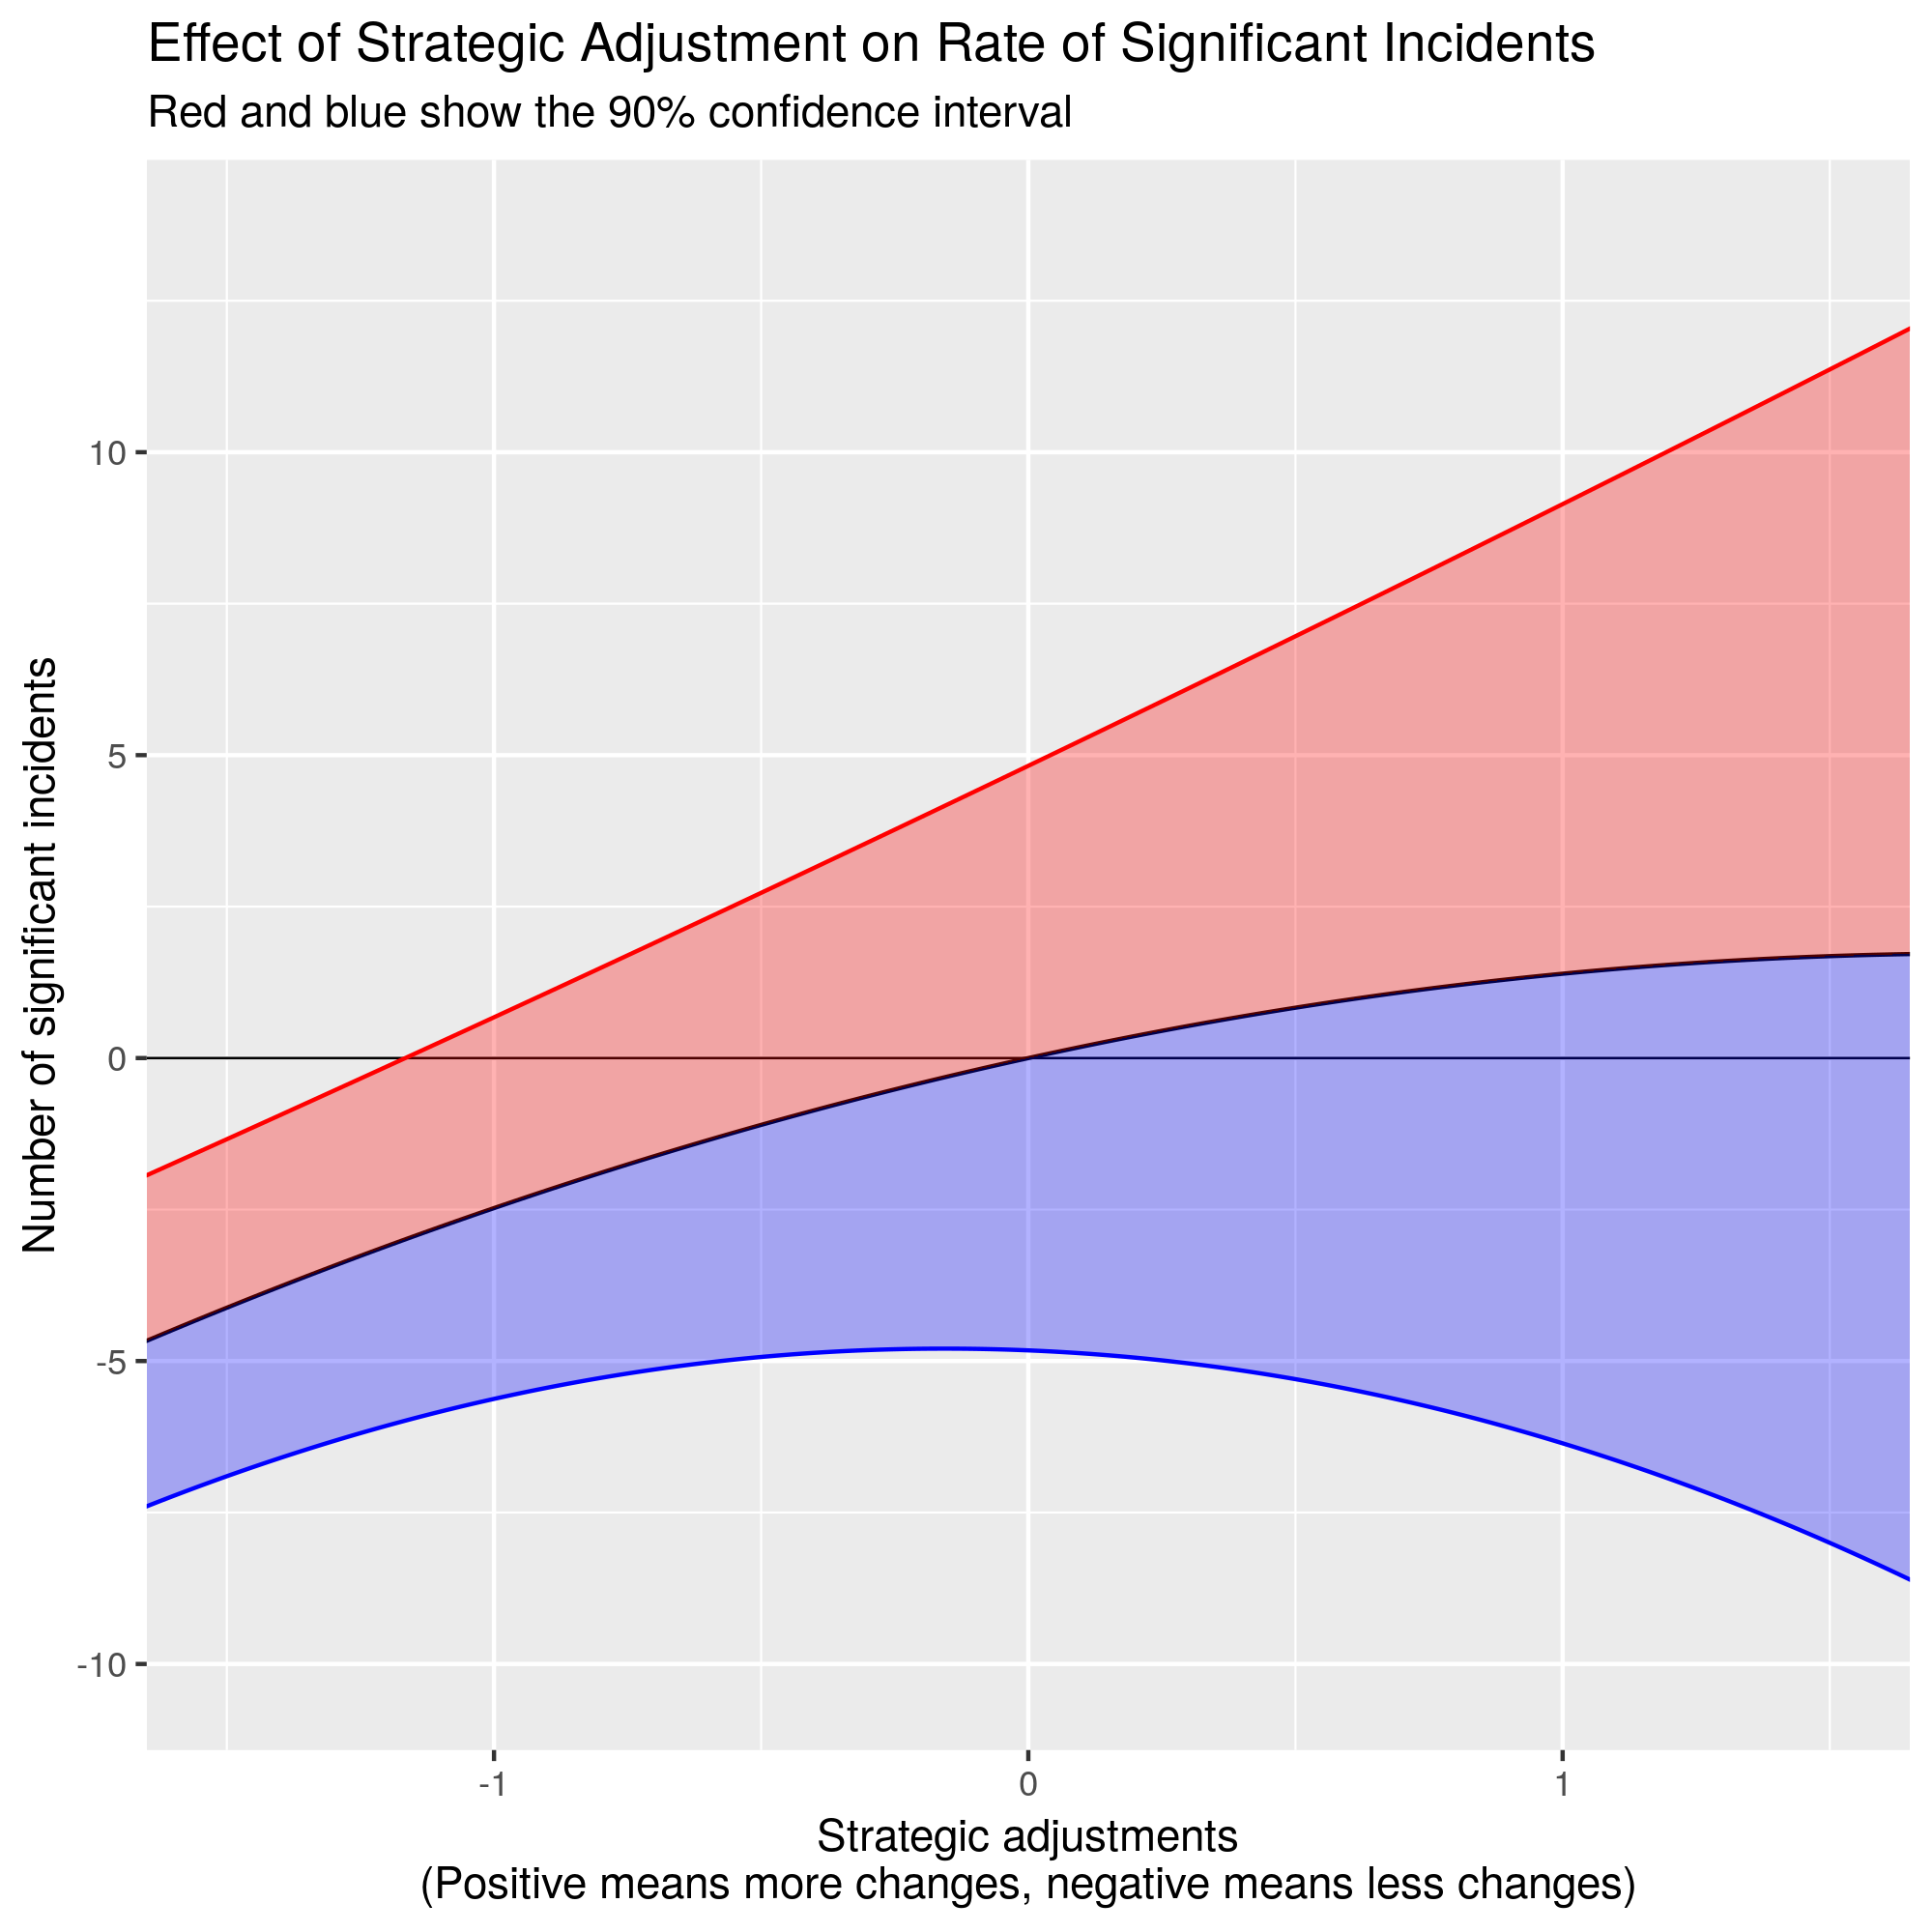
\includegraphics{illustrations/effect_size.png}
	\caption{}
\end{figure}


\section{Conclusion}

\begin{frame}
	\frametitle{Summary}
	\begin{block}{Findings}
		\begin{itemize}
			\item Organization-wide strategic changes will disrupt learning that has occurred in suborganizations.
			\note{This is what expansion mode refers to in the title, not greenfield or M\&A (although there are M\&As in the dataset).\\\medskip}
			\item Thus, when "nothing happens", something does happen: organizational learning.
			\item From a learning perspective, it is better to take a long-term perspective on strategic adjustments.
			\begin{itemize}
				\item Implementing change in a less disruptive fashion.
			\end{itemize}
			\note{"Learning perspective" matters, because from a technology perspective, the conclusion might be different.}
			\item Depending on the context, implications for organizational performance (environmental and economic).
			\note{In a temporality-inspired learning research fashion. Depending on the type of organization - where mistakes threaten survival, very relevant.}
		\end{itemize}
	\end{block}
\end{frame}

\begin{frame}
	\frametitle{Summary}
	\begin{block}{Limitations}
		\begin{itemize}
			\item Not controling for revenue, profitability, number of employees yet.
			\note{Could merge in business unit level data from compustat.\medskip}
			\item Results driven by a number of outliers.
			\note{Already remove most extreme outliers, but have not analyzed this issue further - robustness check?\medskip}
			\item Further disentangle effect of technology vs. strategy.
			\note{Empirical analysis of the two - which dominates?}
		\end{itemize}
	\end{block}
\end{frame}

\begin{frame}[allowframebreaks]
	\frametitle{Bibliography}
	\bibliography{bibliography}
	\bibliographystyle{chicago}
\end{frame}

\end{document}